%%% PREAMBLE - Do not touch %%%%%%%%%%%%%%%%%%%%%%%%%%%%%%%%%%%%%%%%%%%%%%%%%%%%%%
\documentclass[10pt,twocolumn,letterpaper]{article}
\usepackage[utf8]{inputenc}
\usepackage[brazil]{babel}
\usepackage{bm}
\usepackage{model}
\usepackage{times}
\usepackage{epsfig}
\usepackage{graphicx}
\usepackage{amsmath}
\usepackage{amssymb}
\usepackage{color}
\usepackage[pagebackref=true,breaklinks=true,letterpaper=true,colorlinks,bookmarks=false]{hyperref}

\cvprfinalcopy % *** Uncomment this line for the final submission
\def\httilde{\mbox{\tt\raisebox{-.5ex}{\symbol{126}}}}
\ifcvprfinal\pagestyle{empty}\fi

%%% Report beginning %%%%%%%%%%%%%%%%%%%%%%%%%%%%%%%%%%%%%%%%%%%%%%%%%%%%%%%%%%%%%%
\begin{document}

%%% Title and authors %%%%%%%%%%%%%%%%%%%%%%%%%%%%%%%%%%%%%%%%%%%%%%%%%%%%%%%%%%%%
\title {Predizendo o modelo da câmera de uma fotografia a partir de técnicas de aprendizado de máquina}
\author{Gustavo Ciotto Pinton, RA117136\thanks{Is with the Institute of Computing, University of Campinas (Unicamp). \textbf{Contact}: \tt\small{gustavociotto@gmail.com}}}

%%% Abstract %%%%%%%%%%%%%%%%%%%%%%%%%%%%%%%%%%%%%%%%%%%%%%%%%%%%%%%%%%%%%%%%%%%%%
\maketitle
\begin{abstract}
São propostos neste documento dois métodos de classificação baseados em aprendizado de máquina e capazes de determinar, a partir de uma foto, o modelo da câmera que a gerou. No total, 10 modelos de câmeras distintas, mas de mesmos fabricantes, são utilizados neste problema. O primeiro, baseado na técnica de regressão logística, consiste em separar as 10 classes em grupos binários de maneira a testar sempre um dos modelos contra os demais, enquanto que o segundo, baseado em redes neurais, busca diretamente a classe de determinada imagem, sem quaisquer divisão binária dos grupos. Além disso, neste artigo, estão descritos os atributos recuperados das imagens e os parâmetros configurados em cada um dos métodos, bem como a sua influência no resultado final. Por fim, são apresentados os resultados de cada uma das técnicas e o score obtido para o problema na plataforma Kaggle.
\end{abstract}

%%% Introduction %%%%%%%%%%%%%%%%%%%%%%%%%%%%%%%%%%%%%%%%%%%%%%%%%%%%%%%%%%%%%%%%%
\section{Introdução}
\label{intro}

A técnica de regressão logistíca, ao contrário do método de regressão linear cujo objetivo é adequar os dados a uma equação linear, busca classificar os dados de entrada em dois grupos discretos, comumente denominados \(0\) e \(1\). Para tal, define-se a matriz \(\bm{x}\) de dimensões \(N + 1 \times M\)  contendo \(M\) entradas descritas por \(N + 1\) atributos (contando evidentemente um elemento de \textit{bias}), o vetor \(\bm{\theta}\) representando o peso que cada atributo terá no modelo e a uma função \(g\left(\bm{\theta}, \bm{x}^{(i)}\right)\) cujo conjunto imagem é o intervalo \([0,1]\). Esta última é responsável por predizer a classe \(\bm{\hat{y}}^{(i)}\) de cada entrada \(\bm{x}^{(i)}\), tendo em vista que valores \(\bm{\hat{y}}^{(i)}\) mais próximos de 0 indicarão que determinada entrada tem mais chance de pertencer à classe 0 e vice-versa. A função \(g\), a princípio, pode assumir qualquer equação desde que sua imagem fique entre 0 e 1. Para este documento, tal função assumirá a forma sigmoidal, conforme equação \ref{eq:sig}.

\begin{equation}
\label {eq:sig}
\bm{\hat{y}}^{(i)} = g \left(\bm{\theta},\bm{x}^{(i)}\right) = \frac {1}{1 + e^{-\bm{\theta}^T\bm{x}^{(i)}}}
\end{equation}

Neste caso, se \(\theta^T\bm{x}^{(i)}\) é grande, então \(e^{-\theta^T\bm{x}^{(i)}}\) tende a zero e a classe atribuida à entrada \(i\) será 1. Em oposição, se \(\theta^T\bm{x}^{(i)}\) é muito negativo, a função tenderá a 0, assim como a classe escolhida.

Assim como quase toda técnica de aprendizado de máquina, a determinação dos valores do vetor \(\bm{\theta}\) envolve a minimização de uma função de custo \(J(\bm{\theta}, \bm{x})\), descrita pela equação \ref{eq:cost}, a partir de um conjunto de entradas \(\bm{x}^{(i)}\) de saídas \(\bm{y}^{(i)}\) conhecidas.

\begin{equation}
\begin{split}
\label {eq:cost}
J(\bm{\theta}, \bm{x}) = -\frac{1}{M} \displaystyle\sum_{i=1}^{M} & \left[ \bm{y}^{(i)}\log \left( \bm{\hat{y}}^{(i)} \right) + \ldots \right. \\
& \left.  + \left(1 -\bm{y}^{(i)}\right)\log \left(1 - \bm{\hat{y}}^{(i)} \right) \right] \\
\end{split}
\end{equation}

Como visto em aula, a função \(J(\bm{\theta}, \bm{x})\) é convexa e, portanto, não possui mínimos locais além do global e sua minimização pode ser realizada também através do método de \textit {gradient descent}, explorada na última atividade. Os dados utilizados para a minimização \(\bm{x}^{(i)}\) e \(\bm{y}^{(i)}\) pertencem a um conjunto denominado \textbf{conjunto de treinamento}, enquanto que a validação dos parâmetros obtidos ocorre em um conjunto que recebe este mesmo nome. Um regra geral é separar 80\% dos dados disponíveis para treinamento e o restante, 20\%, para testes e validação.

Derivando-se parcialmente a equação \ref{eq:cost} em relação a \(\bm{\theta}_j\), obtém-se o coeficiente linear e portanto a direção que devemos tomar para nos aproximar do mínimo global. Repetindo o raciocínio para todos os parâmetros \(\bm{\theta}_j\), obtém-se à operação \ref{gd} que deve ser aplicada a cada um deles a cada iteração. Observa-se que, apesar de que o cálculo de \ref {eq:sig} ser totalmente diferente da aproximação realizada pelo modelo linear, isto é, \(\bm{\hat{y}}^{(i)}_{lr} = \bm{\theta}^T\bm{x}^{(i)}\), obtemos exatamente a mesma equação para cada iteração, conforme equação \ref{gd}. Assim como explorado na atividade passada, \(\alpha\) é chamado de \textit{learning rate} e controla a velocidade de convergência ao mínimo global.

\begin{equation}
\label {gd}
\bm{\theta}_j = \bm{\theta}_j - \alpha\frac{\partial J}{\partial \bm{\theta}_j } = \bm{\theta}_j - \frac{\alpha}{M} \displaystyle\sum_{i=1}^{M} \left(\bm{\hat{y}}^{(i)} - \bm{y}^{(i)}\right)\bm{x}_j^{(i)}
\end{equation}

É importante observar que, para problemas com mais de duas classes, é necessário adotar estratégias para o uso da regressão logística, tendo em vista que ela é capaz de modelar apenas problemas \textit {binários}. Sendo assim, exploramos duas estratégias durante as aulas. A primeira, chamada de \textit{one vs. all} consiste em obter \(n\) modelos com \(n\) igual o número de classes e, para cada um, calcular \(\bm{\hat{y}}^{(i)}_j\). A classe \(j\) escolhida será aquela com maior \(\bm{\hat{y}}^{(i)}_j\). Na segunda estratégia, denominada \textit{many vs. many}, seleciona-se aleatoriamente grupos de classes e calcula-se um preditor para cada um deles. A determinação da classe ocorre da mesma maneira, isto é, a partir da verificação da maior probalidade. Para este problema, entretanto, escolhe-se a primeira estratégia.

Apesar da relativa facilidade que a regressão logística oferece, problemas que possuem muitos atributos de entrada, tais como o apresentado nesse documento, tendem a não ser bem modelados por essa técnica, devido ao fato de que \(\bm{\theta}^T\bm{x}\) permanece sendo uma relação linear. Pode-se argumentar que é possível gerarmos mais atributos de ordens superiores, porém isso nos conduziria a outros problemas, tais como aumento de complexidade e \textit{overfitting}. É neste cenário que a segunda técnica, baseada em redes neurais, torna-se importante, à medida que é bem-sucedida em capturar as não-linearidades do modelo. As redes neurais são compostas, dependendo de sua arquitetura, de diversas unidades denominadas neurônios, que podem ser enxergadas individualmente como regressores logísticos, organizadas em camadas interligadas entre si. A cada neurônio da camada \(i\), são ligadas \(n_{i-1} + 1\) entradas provindas da camada \(i-1\), multiplicadas pelo vetor de pesos \(\bm{\theta}_{(i-1)}\), gerando um saída \(a_i\), denominada ativação, conforme equação \ref{eq:neuron}. Uma rede neural possui, no mínimo, duas camadas, sendo elas as de entrada e a de saída. As camadas intermediárias, por sua vez, recebem o nome de \textit{hidden layers}.

\begin{equation}
\label {eq:neuron}
a_{i} = g \left(\bm{\theta}_{(i-1)},\bm{x}_{(i-1)}\right) = \frac {1}{1 + e^{-\bm{\theta}_{(i-1)}^T\bm{x}_{(i-1)}}}
\end{equation}

A determinação dos parâmetros \(\bm{\theta}_{(i-1)}\) envolve, assim como no caso da regressão logística, a minimização de um função de custo \(J\). A técnica de \textit{gradient descent} poderia ser evidentemente utilizada, porém ela exigiria muito poder computacional dado a maior complexidade do modelo e a quantidade de parâmetros a ser determinados. Desse modo, uma outra técnica, chamada de \textit{backpropagation} se mostra interessante, à medida que é capaz de estimar o valor da derivada parcial da função \(J\) em relação a cada \(\bm{\theta}_{(i-1)}\) a partir da acumulação dos erros obtidos indo-se da camada \(l+1\) à \(l\).

Para o nosso problema, propõe-se o uso de apenas uma camada intermediária e 10 neurônios da camada de saída, cada um gerando a probabilidade de determinada imagem pertencer a uma das 10 classes.

Tendo visto duas ferramentas de classificação, podemos aplicá-las a dados reais. Neste relatório, usamos dados de uma competição publicada na plataforma \textit{Kaggle}, em que os competitores foram desafiados a determinar o modelo da câmera que gerou determinada fotografia. Em outras palavras, busca-se dividir o conjunto de entrada em 10 classes distintas, cada uma representando um modelo de câmera distinto. No total, 275 fotografias de cada modelo foram disponibilizados para treinamento dos classificadores. Nas próximas seções, serão discutidos o processo de aquisição de atributos das imagens, o processo de treinamento e os resultados obtidos.

%%% Add section %%%%%%%%%%%%%%%%%%%%%%%%%%%%%%%%%%%%%%%%%%%%%%%%%%%%%%%%%%%%%%%%%%
\section{Atividades}

As próximas subseções visam explicar as escolhas dos diversos parâmetros adotados pelo autor.

\subsection{Cálculo dos atributos}

Durante as aulas, discutimos que cada modelo de câmera utiliza seu próprio método de interpolação para cada \textit{pixel} constituindo uma imagem. Em outras palavras, esta informação pode ser vista como a assinatura do equipamento na fotografia. Vimos também que a maneira mais correta de obtermos tal \textit{assinatura} é através do ruído de cada uma das bandas \textit{RGB}, isto é, aplicamos um filtro  \(f\) à imagem \(I\) e subtraímos o resultado da imagem original, conforme equação \ref{eq:noise}.

\begin{equation}
\label{eq:noise}
N = I - f(I)
\end{equation}

Alguns trabalhos \cite{5337441}\cite{6913721} na área apontam que o uso de \textit{discrete wavelet transform} produz melhores resultados na identificação, isto é, os atributos gerados são capazes de traduzir com mais pertinência e significância a \textit{assinatura} em cada fotografia. Baseando-se nestes dois trabalhos citados, foram calculados para cada imagem os seguintes atributos:

\begin{itemize}
  \item Conforme \cite{5337441}, \textbf{média}, \textbf{variância}, \textbf{skewness} e \textbf{kurtosis} das direções horizontal, vertical e diagonal de cada uma das quatro escalas da \textit{discrete wavelet transform} aplicadas em cada uma das bandas \textit{RGB}, resultando, no total, em 144 atributos.
  \item Ainda de acordo com \cite{5337441}, estatísticas da matriz de \textit{co-ocurrence} também foram calculadas. Para as direções horizontal, vertical e diagonal de cada uma das quatro escalas da \textit{discrete wavelet transform} em cada uma das bandas \textit{RGB} e quatro ângulos diferentes, calculou-se a \textbf{energia}, \textbf{entropia}, \textbf{contraste}, \textbf{homogeneidade} e \textbf{correlação}, resultado, assim, em mais 720 atributos.
  \item O processo de obtenção de atributos de \cite{6913721} foi reproduzido, isto é, foram calculados 9 momentos centrais para as três direções de cada uma das quatro escalas da \textit{discrete wavelet transform} aplicada a \(N\). \(N\) foi calculada da mesma maneira que representada em \cite{6913721}. Nesta etapa, gera-se 324 atributos adicionais.
\end{itemize}

No total, gera-se, portanto, 1188 atributos para cada imagem.

\subsection{Ajuste o parâmetro \(\alpha\) da regressão logística}
\label{sec:ajuste}

Para a técnica de \textit{gradient descent}, a estratégia de modificação do parâmetro \(\alpha\) (\textit{learning rate}) é muito importante para impedir eventuais balanços em torno do mínimo global. Como utilizamos uma solução já pronta para a regressão logística, usamos uma das opções disponibilizadas pela biblioteca para tal estratégia. Utilizou-se, assim, aquela denominada \textit{AdaGrad} \cite{Duchi:2011:ASM:1953048.2021068}, ou \textit{adaptive gradient algorithm}, em que diferentes taxas de aprendizado são utilizadas de acordo com os atributos. Alguns atributos podem se mostrar úteis para um problema de otimização, mas podem não aparecer na maioria das entradas de treinamento. Se, quando aparecem, eles são tratados da mesma forma em termos de taxa de aprendizado em relação a um recurso que apareceu centenas de vezes, estamos considerando que a influência de tais atributos não significa nada na otimização geral. A fim de combater este efeito, a estratégia \textit{AdaGrad} faz com que atributos que são mais esparsos nos dados tenham uma taxa de aprendizado maior, o que se traduz, desse modo, em uma atualização maior para esse determinado atributo.

\subsection{Regularização}

A fim de evitar efeitos indesejados gerados devido ao \textit{overfitting}, consideramos para ambas as técnicas o uso de um parâmetro de regularização. Assim como destacado no primeiro exercício, esse parâmetro penaliza os pesos \(\bm{\theta}_j\) impedindo que o modelo gerado apresente pequena variação com as entradas utilizadas no treinamento. Foi determinado experimentalmente o valor de \(\lambda = 10\) para ambas as técnicas.

\subsection {Arquitetura da rede neural}

A rede neural utilizada foi constituída apenas de três camadas: a de entrada com 1188 atributos, a de saída com 10 neurônios, um para cada classe, e apenas uma intermediária com o número de neurônios igual aquele de atributos, isto é, 1188. Esta escolha foi adotada a partir de testes com os conjuntos de treinamento e do fato de que, nesta atividade, não foi visado o uso de \textit{deep neural networks}, isto é, redes com muitas camadas intermediárias. Para cada neurônio, a função \textit{sigmóide} foi utilizada como função de ativação.

%%% Add section %%%%%%%%%%%%%%%%%%%%%%%%%%%%%%%%%%%%%%%%%%%%%%%%%%%%%%%%%%%%%%%%%%
\section{Soluções propostas}

Essa seção é dedicada à discussão das soluções propostas. Foram realizados testes com regressores logistícos e redes neurais. Em todos os casos, usou-se 80\% do conjunto de imagens para treinamento dos modelos e 20\% para validação.

\subsection {Conjunto de treinamento original}

Nesta subseção, serão descritos os resultados obtidos para o conjunto de treinamento de imagens original, isto é, sem quaisquer adições a tal conjunto.

\subsubsection {Regressão logística}

Conforme comentado na seção \ref{intro}, utilizamos a estratégia de \textit{one vs. all} para a classificação das classes. A figura \ref{img:lr1} representa a matriz de confusão resultante do conjunto de validação. Em média, os regressores foram bem sucedidos em predizer a classe de 94.7\% das imagens do conjunto de validação. O modelo que obteve o maior número de erros foi o \textit{HTC 1 M7}. Utilizando o modelo com o conjunto de testes, que é constituído por imagens que foram recortadas e transformadas, tal média caiu para apenas 20.22\%, indicando que o modelo não é capaz de predizer corretamente o modelo de imagens que sofreram algum tipo de alteração.

\begin{figure}
    \centering
    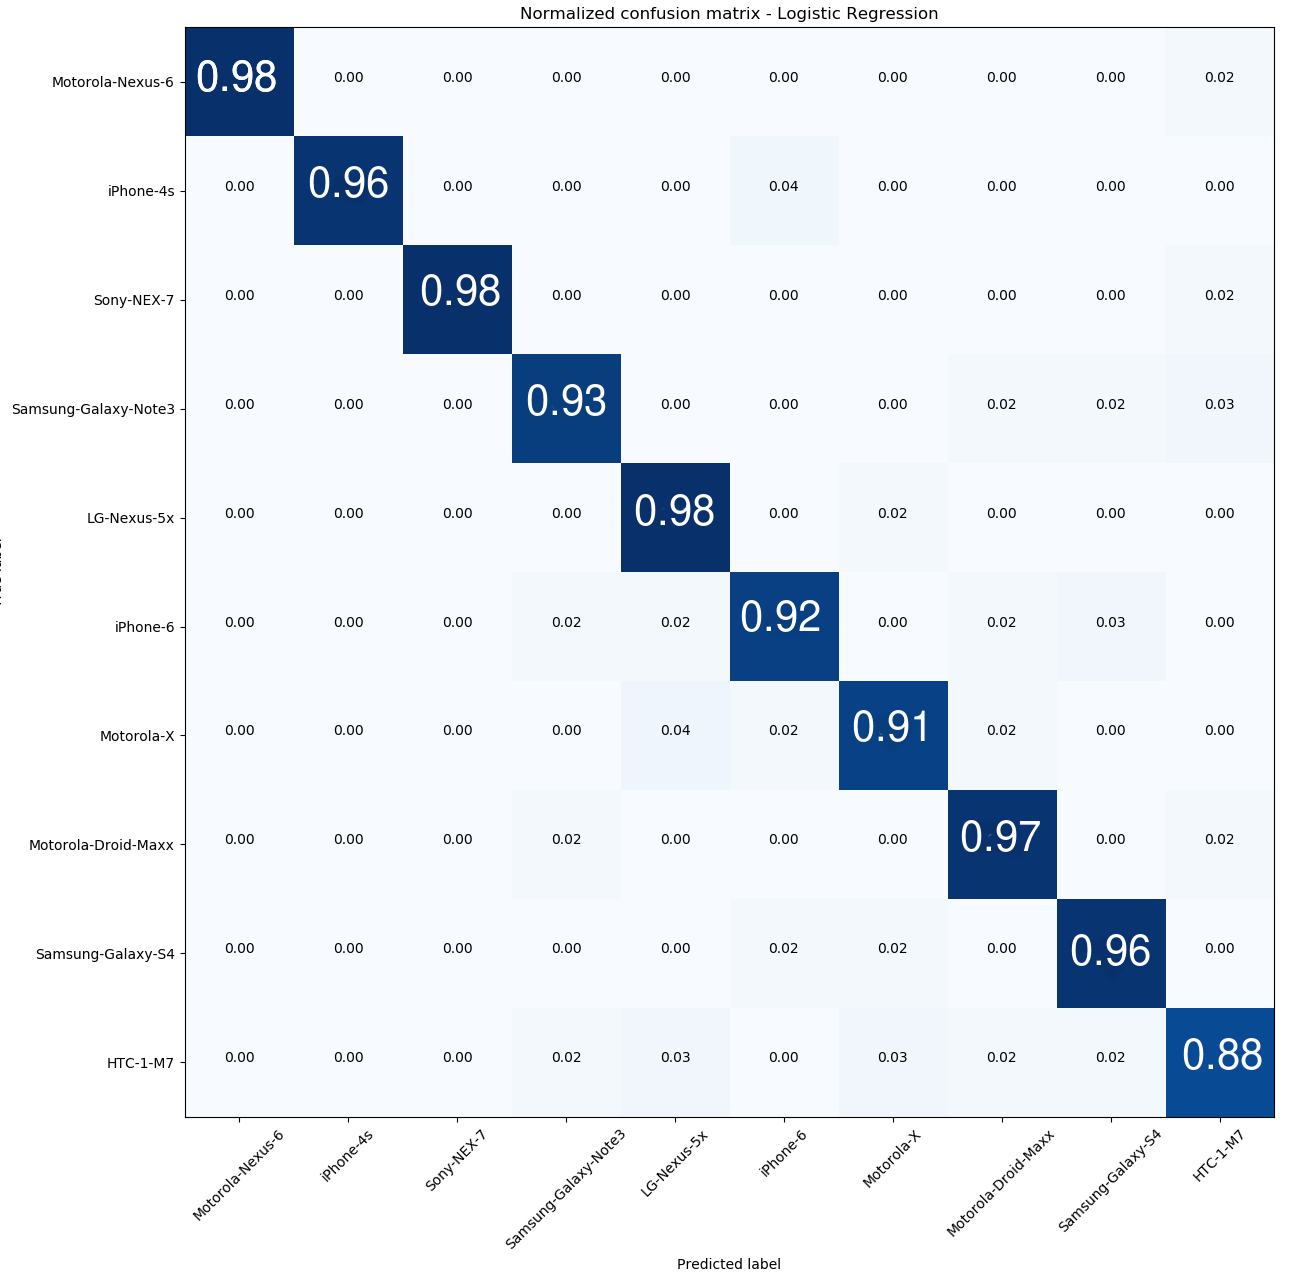
\includegraphics[width=\columnwidth]{images/lr-no_crop.png}
    \caption{Matriz de confusão para a regressão logística. Quanto mais escura uma célula, mais próximo de 1.00 seu conteúdo é.}
    \label{img:lr1}
\end{figure}

\subsubsection {Rede neural}

A figura \label{img:nn1}, por sua vez, reproduz a matriz de confusão para a rede neural. Neste caso, obtém-se um resultado ligeraimente inferior àquele obtido para a regressão logistíca: em média, apenas 81.4\% foram classificadas corretamente. Para quatro modelos, o índice de acerto foi inferior a 80\%, sendo que o pior foi o \textit{Samsung Galaxy S4}, em que um quinto das imagens de validação foram classificadas corretamente. Para a submissão na plataforma \textit{Kaggle}, obteve-se um resultado também inferior, isto é, 17.8\% de acerto.

\begin{figure}
    \centering
    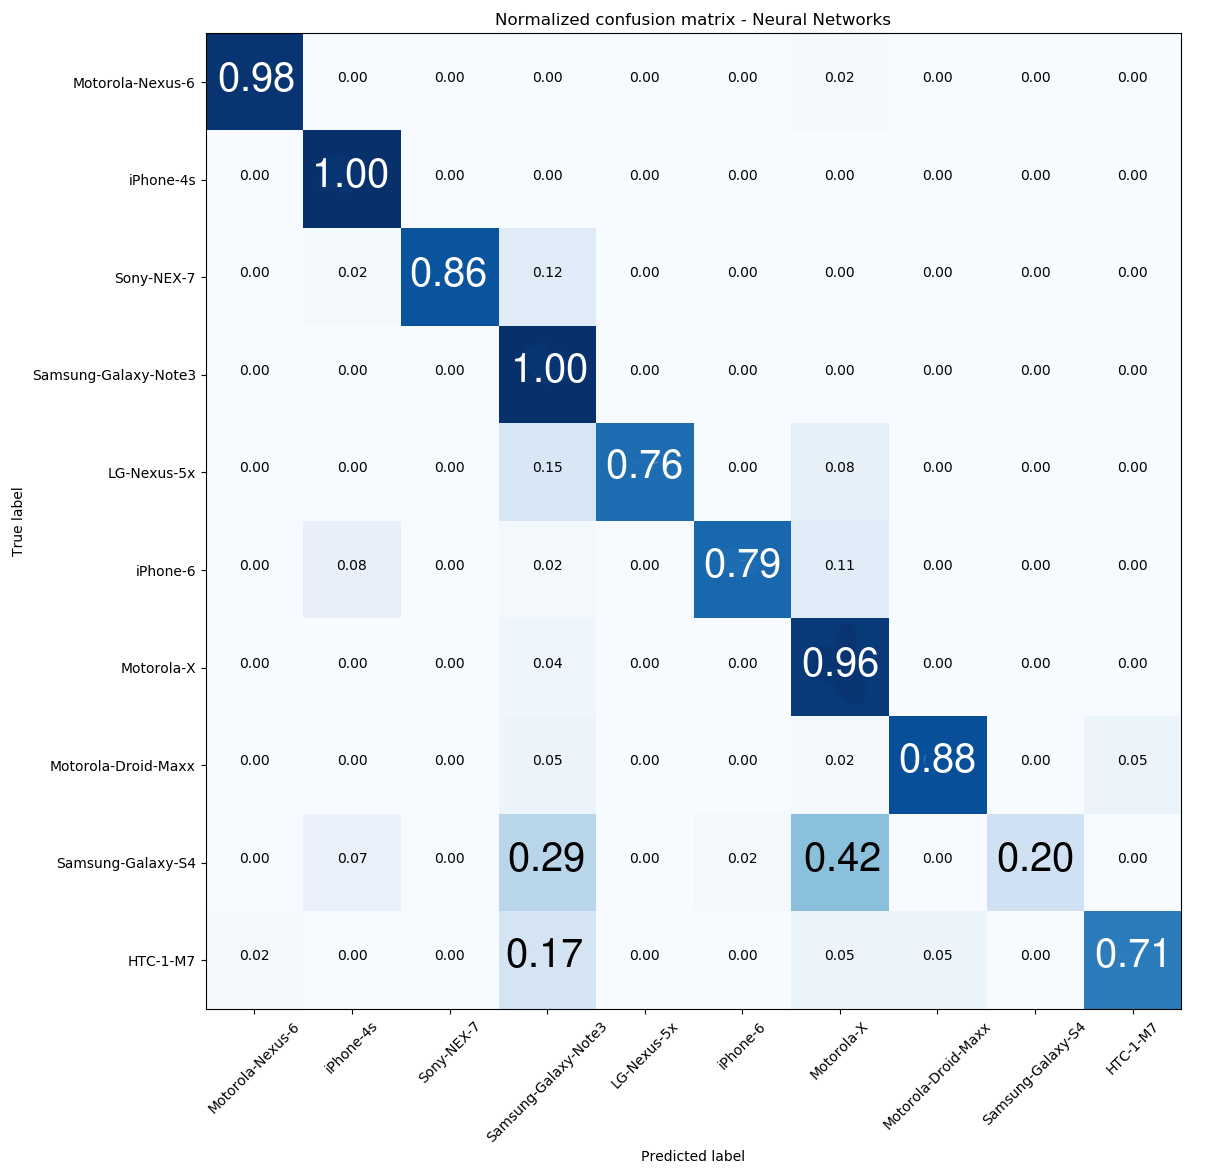
\includegraphics[width=\columnwidth]{images/nn-no_crop.png}
    \caption{Matriz de confusão para a rede neural. Quanto mais escura uma célula, mais próximo de 1.00 seu conteúdo é.}
    \label{img:nn1}
\end{figure}

\subsection {Conjunto de treinamento aumentado}

Tendo em vista os resultados pobres obtidos nas submissões na plataforma \textit{Kaggle}, decidiu-se aumentar o conjunto de imagens de treinamento para incluir imagens de 512x512 recortadas a partir do centro das originais e corregidas em \textit{gamma} com valores de 0.8 e 1.2. Espera-se, portanto, que o índice de acerto para as imagens do conjunto de teste aumente.

\subsubsection {Regressão logística}

A figura \ref{img:lr2} representa a matriz de confusão para a técnica de regressão logística com o conjunto de treinamento aumentado. Neste caso, a média de acerto para as imagens do conjunto de validação cai para 74.7\%, porém a taxa de acerto para o conjunto de testes quase dobra, passando de 20.22\% para 37.4\%. Isto indica que, apesar dos resultados inferiores no conjunto de validação, o modelo está um pouco mais abrangente.

\begin{figure}
    \centering
    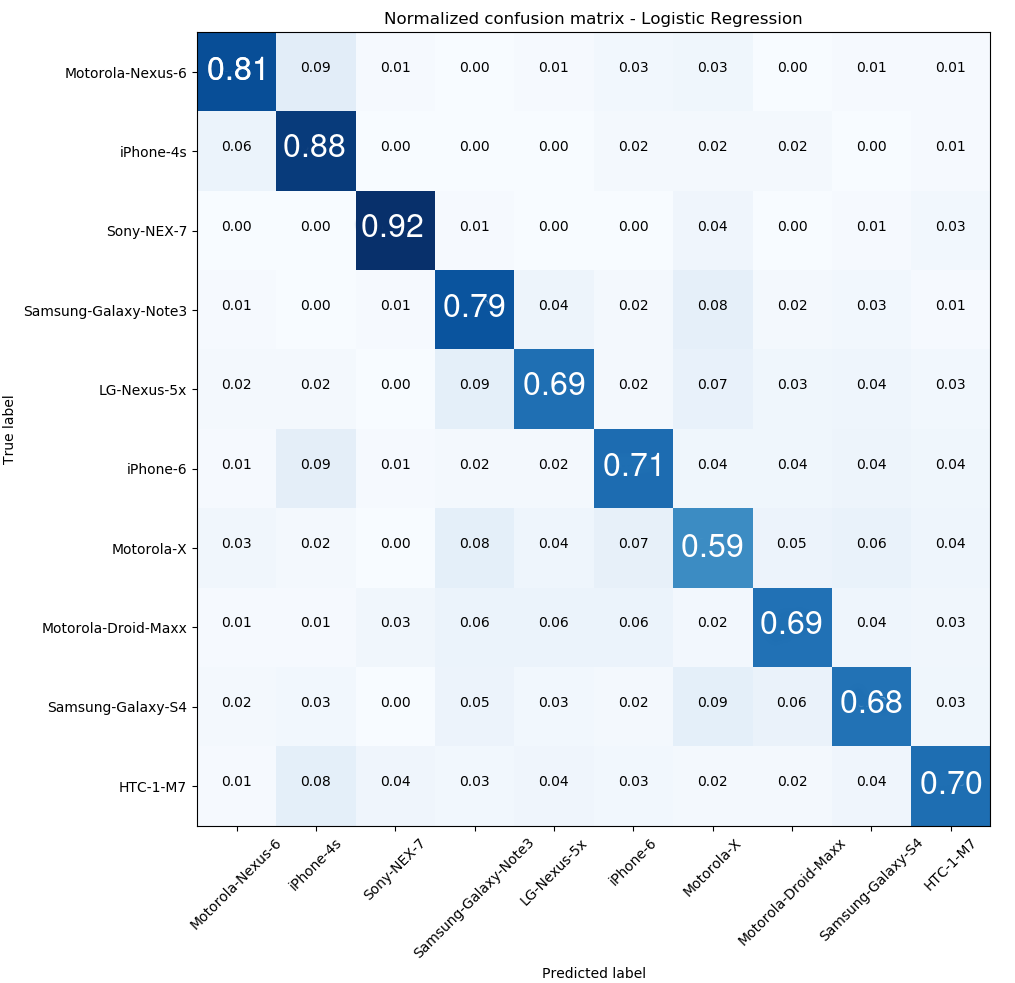
\includegraphics[width=\columnwidth]{images/lr-crop.png}
    \caption{Matriz de confusão para a regressão logística para conjunto de treinamento aumentado. Quanto mais escura uma célula, mais próximo de 1.00 seu conteúdo é.}
    \label{img:lr2}
\end{figure}

\subsubsection {Rede neural}

A rede neural proposta submetida aos novos dados de treinamento produziu uma taxa de acerto, em média, de 52.3\% para o conjunto de validação. Assim como na regressão logística, a acurária obtida na validação foi inferior àquela do caso que utilizou o conjunto de treinamento original, porém a taxa de acerto para o conjunto de teste melhorou, indo de 17.8\% para 25.8\%. Assim como no caso anterior, o modelo tornou-se ligeiramente mais abrangente.

%%% Add section %%%%%%%%%%%%%%%%%%%%%%%%%%%%%%%%%%%%%%%%%%%%%%%%%%%%%%%%%%%%%%%%%%
\section{Conclusões}

Tanto a técnica de regressão logística quanto a de redes neurais obtiveram bons resultados, isto é, acima de 80\% de acerto em média, na classificação das imagens do conjunto de treinamento, porém baixos índices para as imagens modificadas do conjunto de teste. Quando aumentou-se o conjunto de treinamento para considerar algumas das características das imagens presentes no de teste, melhoramos a taxa de acerto em praticamente duas vezes, indicando, portanto, que se quiséssemos aumentá-la ainda mais, teríamos que considerar todas as transformações realizadas no conjunto de teste para o treinamento dos modelos propostos.

%%% References %%%%%%%%%%%%%%%%%%%%%%%%%%%%%%%%%%%%%%%%%%%%%%%%%%%%%%%%%%%%%%%%%%%
{\small
\bibliographystyle{unsrt}
\bibliography{refs}
}

\end{document}
